\section{Theorie}
\label{sec:Theorie}
\subsection{Allgemeine Realaxionsgleichung}
Bei einem System, dass nicht-oszillatorisch in seinen
Ausgangszustand zurückkehrt treten Relaxationserscheinungen
auf. Dabei gilt meist der Zusammenhang
\begin{equation}
    \frac{dA}{dt}=c[A(t)-A(\infty)],
\end{equation}
\noindent wobei A die sich ändernde physikalische Größe ist.
Die Integration dieser Gleichung führt auf die Allgemeine
Relaxationsgleichung
\begin{equation}
    A(t)=A(\infty)+[A(0)-A(\infty)]e^{ct}.
    \label{eq:b}
\end{equation}
\noindent Ist $c$ negativ, und $A$ somit beschränkt,
können mit dieser Formel alle Relaxationsvorgänge beschrieben werden.
\subsection{Entladevorgang eines RC-Kreises}
Ein mit Ladung $Q$ geladener Kondensator erzeugt eine
Kindensatorspannung $U_C$, die einen Strom $I$ bedingt.
Mit Hilfe des Ohmschen Gesetzes lässt sich die
zeitliche Änderung von $Q$ also als
\begin{equation}
    \frac{{\symup{d}\,Q}}{\symup{dt}}=-\frac{1}{RC}\,Q(t)
\end{equation}
schreiben. Mit dem Zusammenhang $Q(\infty) =0$ wird
Gleichung \ref{eq:b} zu
\begin{equation}
    Q(t)=Q(0)\symup{e}^{-\frac{t}{RC}}
\end{equation}
\noindent Die Zeitkonstante $RC$ gibt dabei an, wie
schnell $Q$ seinen Endzustand $Q(\infty)$ erreicht.
Nach $\Delta t=RC$ ändert sich die Ladung $Q$ um
\begin{equation}
    \frac{Q(RC)}{Q(0)}=\frac{1}{\symup{e}},
\end{equation}
\noindent und dem entsprechend auch
\begin{equation}
    \frac{U_C(RC)}{U_C(0)}=\frac{1}{\symup{e}}.
\end{equation}
\subsection{Frequenzabhängigkeiten der Phasenverschiebung und der Amplitude beim Kondensator}
Ein RC-Kreis, der mit Wechselspannung betrieben wird,
kann mit einem mechanischem System verglichen werden,
bei welchem Relaxationsphänomene duch periodische
Auslenkung aus der Gleichgewichtslage auftreten.
Die anliegende äußere Spannung $U$ hat also die Form
\begin{equation}
    U(t)=U_0 \cos (\omega t).
\end{equation}
\noindent Die Kondensatorspannung $U_C$ ist
phasenverschoben zu $U$ und hat die Form
\begin{equation}
    U_C(t)=A(\omega) \cos (\omega t + \phi(\omega)),
\end{equation}
\noindent wobei sowohl die Amplitude $A$ als auch
die Phasenverschiebung $\phi$ von $\omega$
abhängt, also Frequenzabhängig ist. Nach dem zweiten
Kirchhoffschen Gesetz lassen sich die Spannungen
im Stromkreis durch
\begin{equation}
    U_0 \cos (\omega t)=-A\omega RC \sin (\omega t + \phi)+A \cos (\omega t+\phi)
    \label{eq:a}
\end{equation}

\noindent in Zusammenhang setzen. Mit Hilfe dieser
Gleichung und der Überlegung, dass sie zu allen Zeiten 
erfüllt sein muss kann die Phasenverschiebung duch
\begin{equation}
    \phi (\omega)= \arctan (-\omega RC)
\end{equation}
\noindent beschrieben werden. Duch den Zusammenhang
$\omega$=1/$RC$ ergibt sich außerdem die Amplitude als
\begin{equation}
    A(\omega)=\frac{U_0}{\sqrt{1+\omega^2 R^2 C^2}}.
\end{equation}
\noindent Es ist zu erkennen, dass für
$\omega \to 0$ die Phasenverschiebung $\phi$ verschwindet
und $A$ sich $U_0$ annähert. Für $\omega \to \infty$
nähert sich $\phi$ $\pi$/2 an und $A$ geht gegen 0.

Bei diesem Versuch wird die Phasenverschiebung $\phi$
über die Größen a und b bestimmt, wobei b die Periodendauer
einer Schwingung und a die Verrückung zweier Spannungen
bei einem Zweikanaloszillographen ist.
\begin{equation}
    \phi=\frac{a}{b}\cdot2\pi
\end{equation}
\begin{figure}
    \centering
    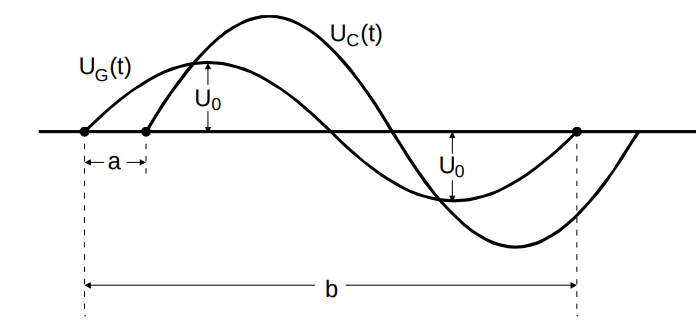
\includegraphics[width=10cm]{content/ab.png}
    \caption{Die Größen a und b bei $U_G(t)$ und $U_C(t)$ \cite{sample}}
\end{figure}

\subsection{Ein RC-Kreis als Integrierglied}
Ein RC-Kreis kann auch als Integrator für die
Wechselspannung $U(t)$ dienen. Gleichung \ref{eq:a} kann
auch als
\begin{equation}
    U(t)=RC \, \frac{\symup{d}\,U_C}{\symup{dt}}+U_C(t)
\end{equation}

\noindent geschrieben werden. Unter der Vorraussetzung
$\omega \gg 1$/$RC$ ergibt sich dann
\begin{equation}
    U(t)=RC \, \frac{\symup{d}\,U_C}{\symup{dt}} \iff U_C=\frac{1}{RC}\int_0^t U(t')\,\symup{d}t'
\end{equation}
